Como Trabajo Terminal, se construirá un robot móvil autónomo, con la capacidad de reconocer el carril por el que se desplaza mediante visión artificial; como lo haría un vehículo real que es operado por un humano. Para validar este robot móvil, se plantea la construcción de una pista de pruebas. En la Figura \ref{fig:PPruebas}, se muestra la propuesta de pista de pruebas de un carril, plana y sin inclinación, en la que se pueden incorporar las señales de tránsito de vuelta a la derecha, vuelta a la izquierda, alto y un semáforo. La pista se plantea reconfigurable, con la posibilidad de cambiar la colocación de los señalamientos para validar la autonomía a través de distintas trayectorias. En esta ilustración, la línea roja representa una de las posibles trayectorias, mientras que los triángulos definen las localizaciones de las señales, mismas características que se pueden distribuir para tener trayectorias distintas. Las medidas finales de la pista están relacionadas con las dimensiones del vehículo, considerando, por ejemplo, el radio de giro.
\begin{figure}[htbp!]
	\centering
	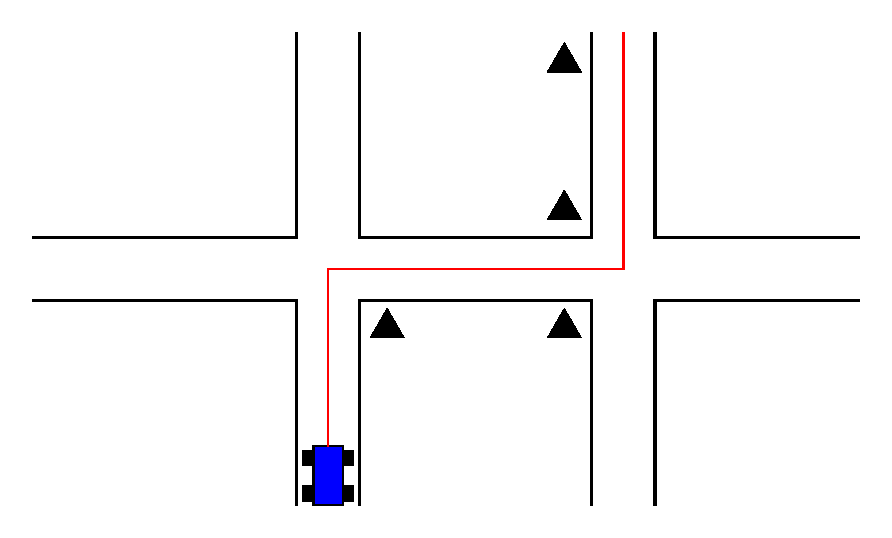
\includegraphics[width=0.6\textwidth]{./Figuras/Pista/Pista}
	\caption{Pista de pruebas propuesta.}
	\label{fig:PPruebas}
\end{figure}
\par A priori, se plantea que esta plataforma móvil usará una configuración Ackerman, por el uso de la misma en vehículos de tamaño real. En el proyecto {\it AutoNOMOS Model} se cuenta con un chasís de un vehículo a control remoto que ha sido adaptado para portar los módulos sensoriales y de cómputo; por su efectividad comprobada, el empleo de algún chasís comercial es opción en la implementación, así como el partir de un chasís de diseño {\it Open-source}. Independientemente de la solución encontrada, se realizarán los análisis y simulaciones que permitirán aprovechar las cualidades intrínsecas de la plataforma, permitiendo además obtener parámetros de funcionamiento que servirán al momento de implementar el control del sistema.
\par Debido a que el proyecto se centra en el diseño e implementación de algoritmos para la conducción autónoma en escenarios urbanos a escala, por la amplitud del proyecto no se trabajará en la descripción de hardware ni la programación a bajo nivel, con lo cual se descarta la posibilidad de usar FPGA\footnote{Por sus siglas en inglés Field-Programable Gate Array} o DSP\footnote{Por sus siglas en inglés Digital Signal Processor}; con lo cual, una arquitectura que resulta cómoda por su compatibilidad con sistemas operativos Linux, es la ARM con ayuda de las computadoras de placa reducida de bajo costo, como las que han emergido en los años recientes, tomando con fines ilustrativos a la Raspberry Pi \cite{foundationRaspberryPiTeach}, Orange Pi \cite{OrangePiOrangepi}, Banana Pi \cite{BananaPiBPI} u Odroid \cite{ODROID}.\\
Para la realización de este proyecto, en la parte de software, se propone usar las librerías OpenCV \cite{opencvOpenCVReferenceManual} y OpenNI \cite{openniOpenNIProgrammerGuide} con el lenguaje de programación C++, por la compatibilidad existente con los sistemas operativos Linux sobre las arquitecturas mencionadas con anterioridad, y con diversos sensores RGB-D del mercado, como el Kinect \cite{InformacionSensorKinect}, el Asus Xtion \cite{XtionPROLIVE}, el Intel RealSense \cite{TecnologiaIntelRealSense}, o el Orbbec Astra \cite{gordonAstraSeries}. 